\documentclass{ieeeaccess}
\usepackage{cite}
\usepackage{amsmath,amssymb,amsfonts}
\usepackage{algorithmic}
\usepackage{graphicx}
\usepackage{units}
\usepackage{color}
\usepackage{textcomp}
\usepackage{caption}
\usepackage{etoolbox}
\usepackage{placeins}
\usepackage{tikz}

% Needed to fix tikz used in ieeeaccess class.
\NewSpotColorSpace{PANTONE}
\AddSpotColor{PANTONE} {PANTONE3015C} {PANTONE\SpotSpace 3015\SpotSpace C} {1 0.3 0 0.2}
\SetPageColorSpace{PANTONE}%

\usetikzlibrary{shapes,arrows}
\tikzstyle{decision} = [diamond, draw, fill=blue!20, 
    text width=4.5em, text badly centered, node distance=3cm, inner sep=0pt]
\tikzstyle{block} = [rectangle, draw, fill=blue!20, 
    text width=5em, text centered, rounded corners, minimum height=4em]
\tikzstyle{line} = [draw, -latex']
\tikzstyle{cloud} = [draw, ellipse,fill=red!20, text width=5em, text centered, node distance=3cm,
    minimum height=2em]

\begin{document}

\history{Date of current version June 25, 2020.}
\doi{PLACEHOLDER}

\title{EEET 4075 Mechatronic System Design 2 - Project Report}
\author{\uppercase{Michael J. Duke}\authorrefmark{1}}
\address[1]{University of South Australia, Mawson Lakes, SA 5095 Australia (e-mail: dukmj002@mymail.unisa.edu.au)}
\tfootnote{This work was supported in part by the University of South Australia}

\markboth
{Michael J. Duke: EEET 4075 Mechatronic System Design 2 - Project Report}
{Michael J. Duke: EEET 4075 Mechatronic System Design 2 - Project Report}

\begin{abstract}
To determine an absolute position and orientation of a robot is not a simple task. Every sensor is subject to noise and errors of some sort, even systems such as the Global Navigation System used in many systems today is subject to large amount of noise and error, making their direct usage less useful. To overcome this, this report demonstrates a method which combines an instantaneous, fast updating, inertia and wheel encoder based estimate, with a slower, delayed beacon based reference position. These estimates are fused using an Extended Kalman Filter (EKF) which is modified to account for the delayed, multirate, multisensor system that is used by incorporating Alexander's Method. The results showed that while the modified EKF worked quite well in and of itself, despite a relatively low update rate, systemic errors introduced in the absolute position reference caused a fair amount of error while traveling at higher velocities.
\end{abstract}

\begin{keywords}
Dead reckoning, Distance measurement, Indoor navigation, Kalman filters, Nonlinear filters, Robot motion.
\end{keywords}

\titlepgskip=-15pt

\maketitle

\section{Introduction}
\label{sec:introduction}
	\PARstart{M}{ultirate} Extended Kalman Filters and absolute versus relative (dead reckoning) localisation.

\section{Related Works}
\label{sec:rel}
	\cite{multi} has infor on multirate, multisensor data fusion. Extracted info includes being able to cascade EKFs into each other indefinitely to allow for many sensors and rates to be included. \cite{indoor} is more for lidar and imu based navigation, used for comparison more than anything. \cite{delayed} specifies different ways to fuse delayed measurements together. \cite{alex} explains the specific method in detail from its creator. \cite{beacon} has information regarding beacon based navigation and triangulation.\par

Several different ways to combine the estimations of different sensors, difficulties with multi-rate systems. Variants or modifications on EKF and UKF, compare and contrast, computational cost, relative accuracy, limitations. maybe compare to particle filters as well? Need for an initial estimate of position and heading. Beacon based navigation.\par
	Using Alexander's Method for fusion of absolute and dead reckoning system due to update rate of LiDaR being much slower than that of odometry and IMU.

\section{Methodology}
\label{sec:meth}
	\subsection{System Model}
	As with most things in control theory, the first step is to determine the state transition model of the system. In the case of the TurtleBot, a lot of the lower level control over the robot is controlled directly by the servomotors themselves. The only variables that are able to be controlled are linear velocity in the x-direction of the bot's local frame $\left(v\right)$, and angular velocity around the z-axis of the bot's local frame $\left(\omega\right)$. As such, the model in \ref{eq:xsys} was developed, where $T$ is the sample period. This model uses a few assumptions and holonomic constraints to keep the model simple.\par
	\begin{itemize}
		\item The robot cannot move sideways or vertically.
		\item The wheels will never slip.
		\item The effects of inertia are negligible.
	\end{itemize}

	\begin{equation}
	\label{eq:xsys}
		\boldsymbol{x}_{ k} = 
		\begin{bmatrix}
			x _{ k}	\\
			y_{ k}		\\
			\theta_{ k}
		\end{bmatrix}
		=
		\begin{bmatrix}
			x_{k-1}+Tv\cos{\left(\theta_{k-1}\right)}								\\
			y_{k-1}+Tv\sin{\left(\theta_{k-1}\right)}								\\
			\theta_{k-1} + T\omega
		\end{bmatrix}
	\end{equation}
	
	With the non-linear system model created, the Jacobian in \ref{eq:Fsys} was calculated to be used for gain and error calculation by the EKF.
	\begin{equation}
	\label{eq:Fsys}
		\boldsymbol{F}_{k} = \frac{\partial\boldsymbol{f}}{\partial\boldsymbol{x_{k-1}}}
		=
		\begin{bmatrix}
			1	&0	&-Tv\sin{\left(\theta_{k-1}\right)}	\\
			0	&1	&Tv\cos{\left(\theta_{k-1}\right)}	\\
			0	&0	&1
		\end{bmatrix}
	\end{equation}

\subsection{Dead Reckoning}
	With the state transition model taken care of, the observation model can be determined. In the case of this EKF, there is two observation models which will be referred as the primary observation model, which includes all of the faster dead reckoning measurements, and the secondary observation model, which includes the slower, absolute measurements.\par
	The primary observation model in this implementation includes information taken from the \textit{joint\_states} topic and the \textit{imu} topic. The \textit{joint\_states} topic has information regarding the position, velocity, and torque of each wheel. For the observation model, only the wheel positions ($s_{l}$ and $s_{r}$) are used. The \textit{imu} topic has information regarding the linear acceleration, angular velocity, and magnetic field orientation of the bot. For the observation model, only the angular velocity around the z axis was used, while acceleration was considered initially, due to the noise, and need for double integration for it to be used, it was not used. for $s_{l}$ and $s_{r}$ to be usable, a small amount of processing is used to convert the information to the change in distance traveled $\left(\delta s_{k}\right)$ and the change of yaw $\left(\delta \theta_{k}\right)$, this is reflected in \ref{eq:delts} and \ref{eq:deltth} and visualized in figure \ref{fig:der}.\par
	\begin{equation}
	\label{eq:delts}
		\delta s_{k} = \frac{\left(s_{r,k} - s_{r,k-1} + s_{l,k} - s_{l,k-1}\right)r}{2}
	\end{equation}
	
	\begin{equation}
	\label{eq:deltth}
		\delta \theta_{k} = \frac{\left(s_{r,k} - s_{r,k-1} + s_{l,k} - s_{l,k-1}\right)r}{b}
	\end{equation}
	Where $b$ is the wheelbase and $r$ is the radius of the wheels, both in meters.
	\begin{equation}
	\label{eq:b}
		b = 0.287
	\end{equation}
	\begin{equation}
	\label{eq:r}
		r = 0.033
	\end{equation}
	
	\begin{figure}
	    	\captionsetup{width=\columnwidth}
	   	\centering
	   	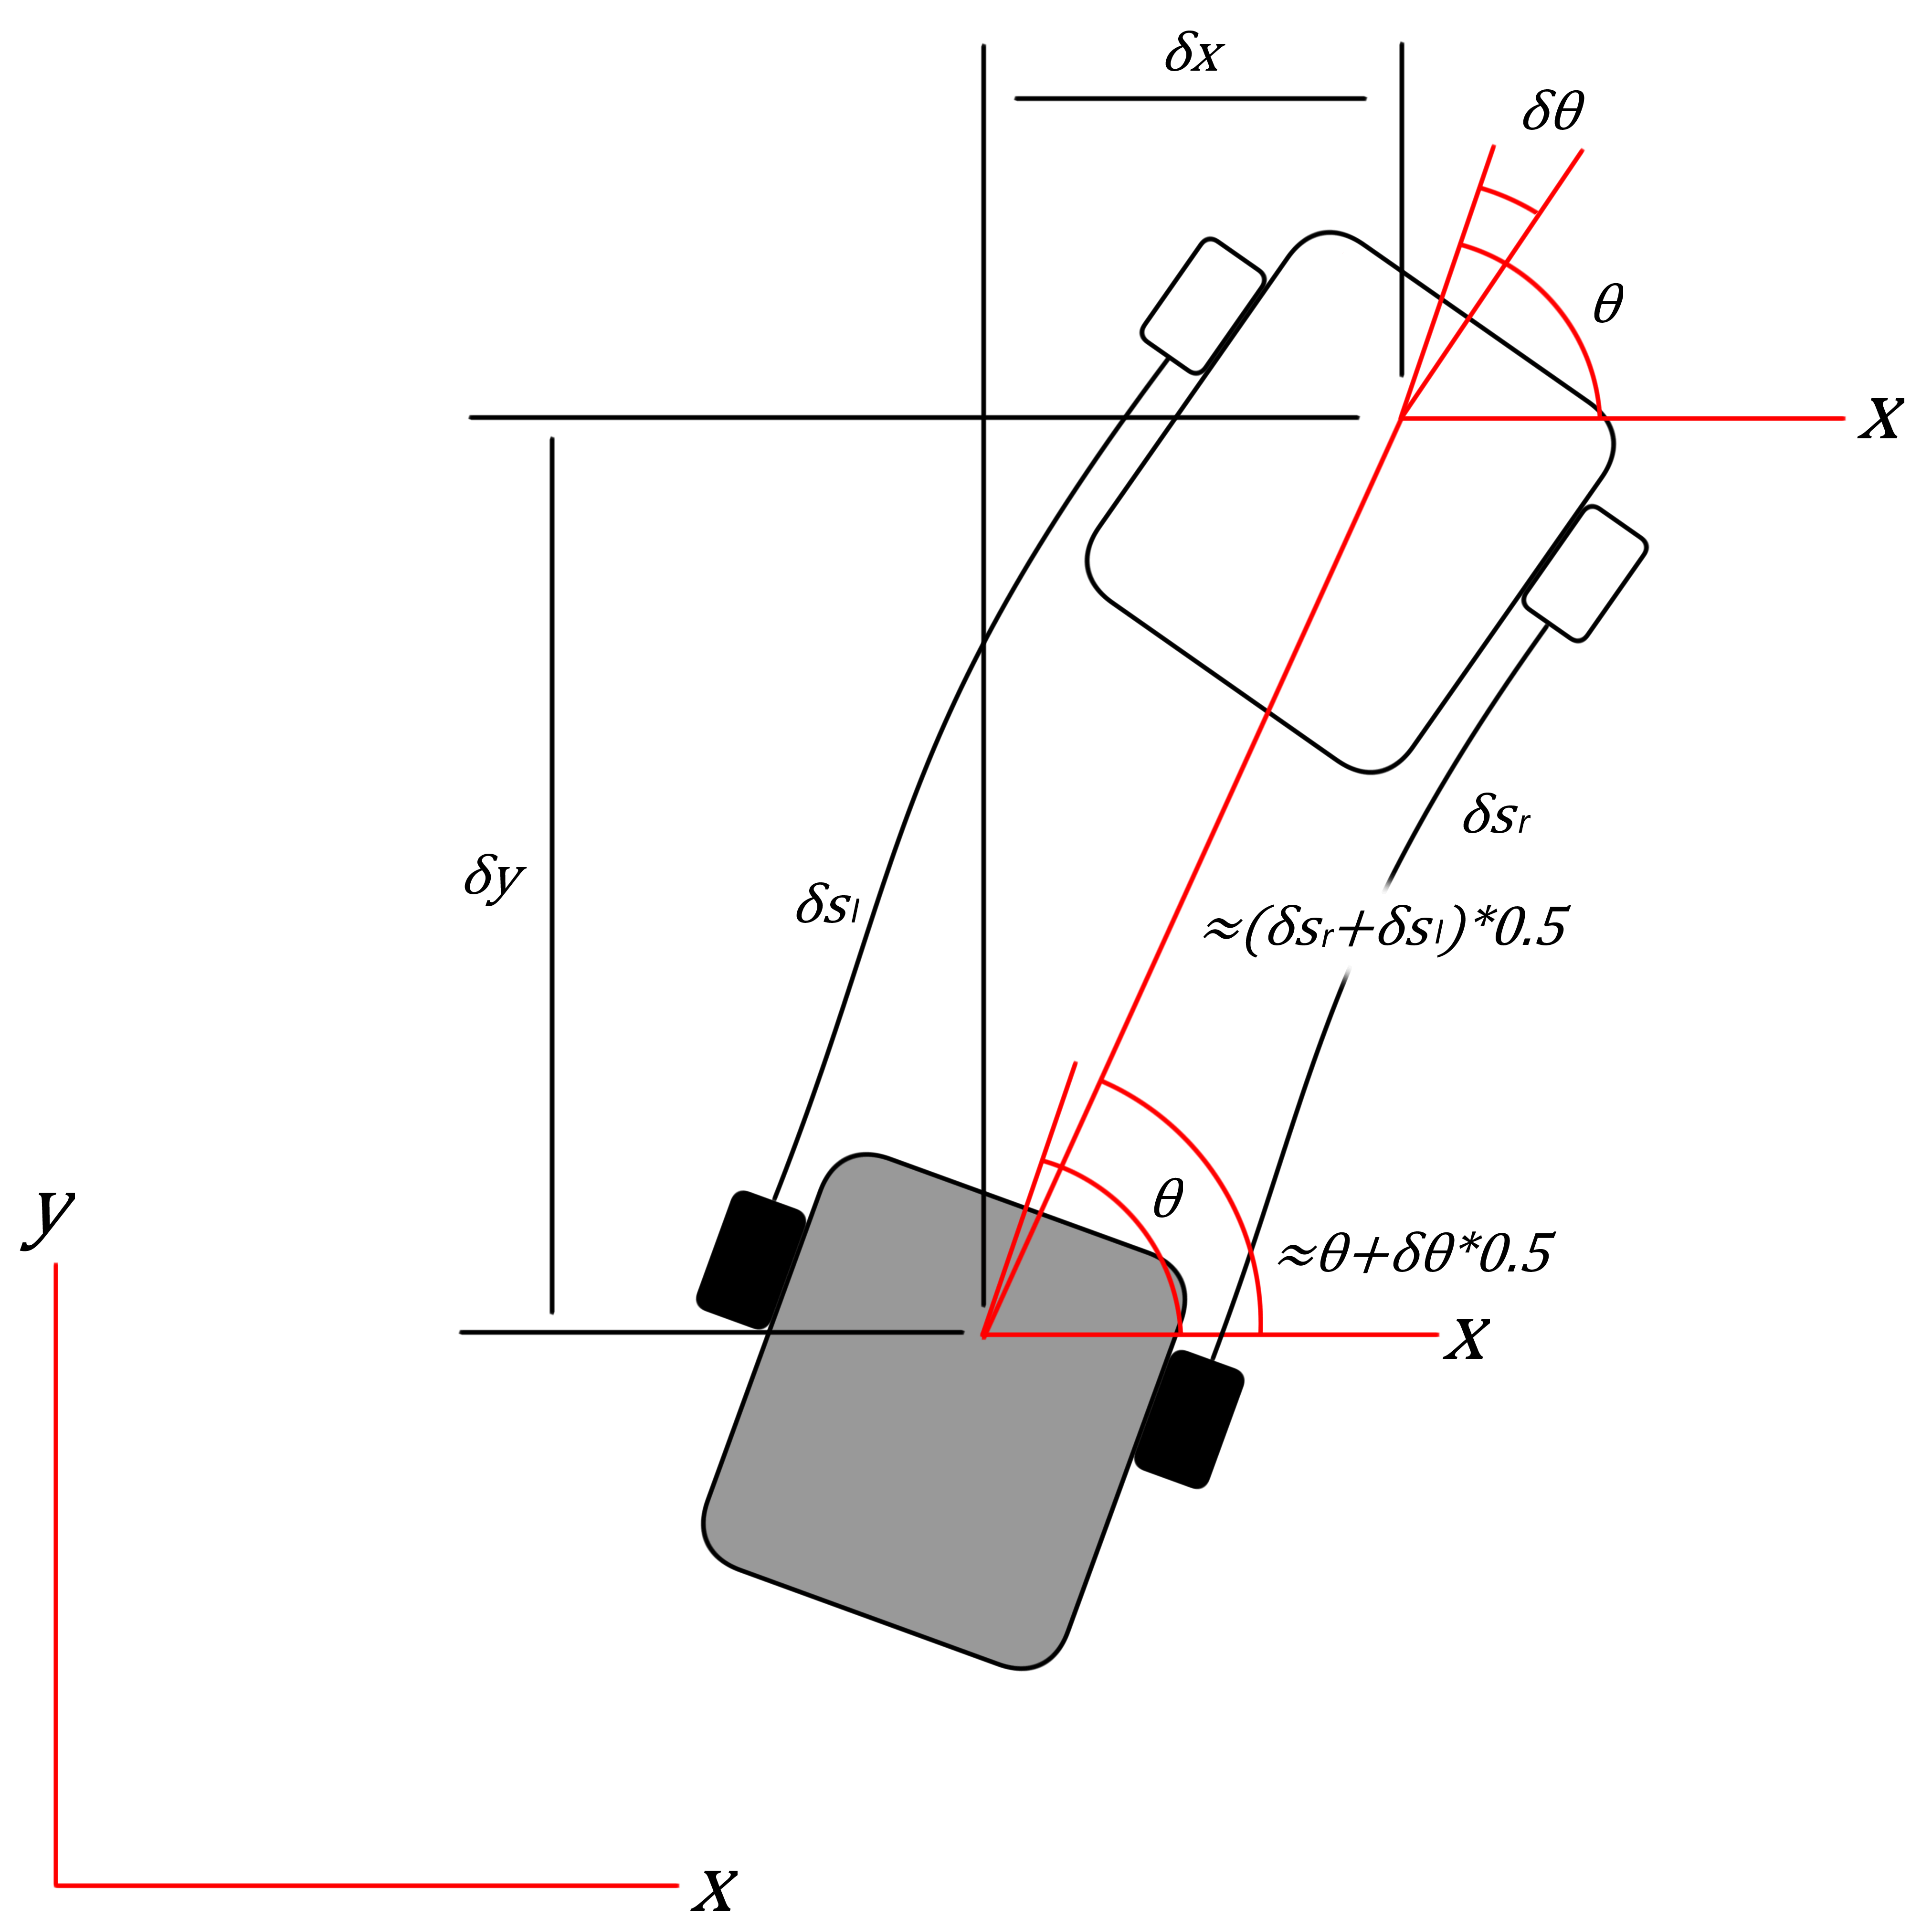
\includegraphics[width=\columnwidth]{./graphics/derive_1.png}
	   	\caption{Geometric estimation of $\delta \theta$, $\delta x$, and $\delta y$ based off $\delta s_{r}$ and $\delta s_{l}$.}
		\label{fig:der}
	\end{figure}
	
	The angular velocity measurement from the \textit{imu} topic $\left(\omega_{k}\right)$ can be used directly. Similar to the state transition model, both the non-linear model and the Jacobian of that model is needed for the EKF, which are presented in \ref{eq:hsys} and \ref{eq:Hsys} respectively.
	\begin{equation}
	\label{eq:hsys}
		\boldsymbol{h}_{ k} =
		\begin{bmatrix}
			\delta s_{k} 		\\
			\delta\theta_{k}	\\
			\omega_{k}
		\end{bmatrix}
		=
		\begin{bmatrix}
			\sqrt{\left(x_{k} - x_{k-1}\right)^{2} + \left(y_{k} - y_{k-1}\right)^{2}}	\\
			\theta_{k} - \theta_{k-1}								\\
			\frac{\theta_{k}-\theta_{k-1}}{T}
		\end{bmatrix}
	\end{equation}
	
	\begin{equation}
	\label{eq:Hsys}
		\boldsymbol{H}_{k}	^{\top}=
		\begin{bmatrix}
			\frac{x_{k}-x_{k-1}}{\sqrt{\left( x_{k} - x_{k-1} \right)^{2}+\left( y_{k} - y_{k-1} \right)^{2}}}	&0	&0		\\
			\frac{y_{k}-y_{k-1}}{\sqrt{\left( x_{k} - x_{k-1} \right)^{2}+\left( y_{k} - y_{k-1} \right)^{2}}}	&0	&0		\\
			0															&1	&\frac{1}{T}
			
		\end{bmatrix}
	\end{equation}

\subsection{Absolute}
	The secondary measurement was implemented as a beacon based navigation system with a method similar to \cite{beacon}. The main difference being that the number of beacons being measured is limited to only two. This is done to reduce the computation time at the expense of accuracy. The method used also does not allow for a definite single estimation position, but a pair of them. With the appropriate assumptions and control measures in place though, one of the positions can always be ruled out.\par
	To estimate the orientation of the turtlebot, the angle to the closest beacon is used as a correction.
	
	To estimate the position of the turtlebot, the intersection of two circles is calculated knowing their center coordinates and radii.
	\begin{equation}
	\begin{aligned}
		\left(x-x_{1}\right)^{2} + \left(y-y_{1}\right)^{2}=r_{1}^{2}	\\
		\left(x-x_{2}\right)^{2} + \left(y-y_{2}\right)^{2}=r_{2}^{2}
	\end{aligned}
	\end{equation}
	Rearranging, and with the assumption that $x_{1}=x_{2}$  in both cases we get
	\begin{equation}
		y = -\frac{r_{1}^{2}-r_{2}^{2}-y_{1}^{2}+y_{2}^{2}}{2\left(y_{1}-y_{2}\right)}
	\end{equation}
	
	\begin{equation}
		x 		= \pm \frac{\sqrt{\beta_{1}\beta_{2}}}{2\left(y_{1}-y_{2}\right)}
	\end{equation}
	\begin{equation}
		\beta_{1} 	= \left(r_{1}+r_{2}+y_{1}-y_{1}\right)\left(r_{1}+r_{2}-y_{1}+y_{1}\right)
	\end{equation}
	\begin{equation}
		\beta_{2} 	=\left(r_{1}-r_{2}+y_{1}-y_{1}\right)\left(-r_{1}+r_{2}+y_{1}-y_{1}\right)
	\end{equation}
	As we know the fence around which the bot cannot escape, one of the possible positions can be eliminated, leaving BLAH if using the left beacons, and BLAH if using the right beacons.
	\begin{equation}
		x 		= x_{1}+\frac{\sqrt{\beta_{1}\beta_{2}}}{2\left(y_{1}-y_{2}\right)}
	\end{equation}
	\begin{equation}
		x 		= x_{1}-\frac{\sqrt{\beta_{1}\beta_{2}}}{2\left(y_{1}-y_{2}\right)}
	\end{equation}
	
	\begin{figure}
	\centering
	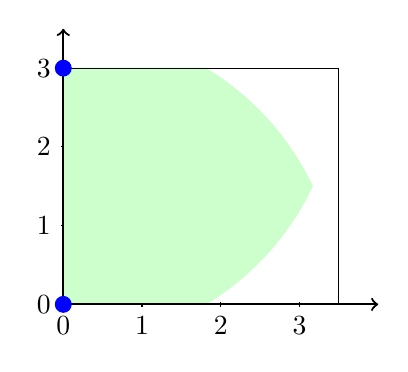
\begin{tikzpicture}
		\foreach \x in {0,1,2,3}
 			\draw (\x cm,1pt) -- (\x cm,-1pt) node[anchor=north] {$\x$};
		\foreach \y in {0,1,2,3}
			\draw (1pt,\y cm) -- (-1pt,\y cm) node[anchor=east] {$\y$};
		\filldraw[fill=green!20!white, green!20!white] (0,0) -- (0,3) -- ({sqrt(3.5^2-3^2)},3) arc ({90-acos(3/3.5)}:{asin(1.5/3.5)}:3.5) arc ({360-asin(1.5/3.5)}:{270+acos(3/3.5)}:3.5);
		\draw (0,0) -- (3.5,0) -- (3.5,3) -- (0,3) -- (0,0);
		\draw[thick,->] (0,0) -- (4,0);
		\draw[thick,->] (0,0) -- (0,3.5);
		\filldraw[fill=blue, blue] (0,0) circle (0.1cm);
		\filldraw[fill=blue, blue] (0,3) circle (0.1cm);
	\end{tikzpicture}
		\label{fig:beac1}
		\caption{Left beacons showing measurable locations in green.}
	\end{figure}
	
	\begin{equation}
		\boldsymbol{h}_{ k} =
		\begin{bmatrix}
			\hat{x}_{k} 		\\
			\hat{y}_{k}		\\
			\hat{\theta}_{k}
		\end{bmatrix}
		=
		\begin{bmatrix}
			x_{k}		\\
			y_{k}		\\
			\theta_{k}
		\end{bmatrix}
	\end{equation}
	
	\begin{equation}
		\boldsymbol{H}_{k} =
		\begin{bmatrix}
			1	& 0	& 0	\\
			0	& 1	& 0	\\
			0	& 0	& 1
		\end{bmatrix}
	\end{equation}
	
	
\subsection{EKF}

	a priori estimate
	\begin{equation}
	\label{eq:x-}
		\hat{\boldsymbol{x}}_{k}^{-}=\boldsymbol{f}_{k-1}\left(\hat{\boldsymbol{x}}^{+}_{k-1},\,\boldsymbol{u}_{k-1}\right)
	\end{equation}
	
	\begin{equation}
	\label{eq:P+}
		\boldsymbol{P}_{k}^{-} = \boldsymbol{F}_{k-1}\boldsymbol{P}_{k-1}^{+}\boldsymbol{F}_{k-1}^{\top} + \boldsymbol{Q}_{k-1}
	\end{equation}
	
	Kalman gain update,
	\begin{equation}
	\label{eq:K}
		\boldsymbol{K}_{1,\,k} = \boldsymbol{P}_{k}^{-}\boldsymbol{H}_{1,\,k}^{\top}\left(\boldsymbol{H}_{1,\,k}\boldsymbol{P}{1,\,k}^{-}\boldsymbol{H}_{1,\,k}^{\top} + \boldsymbol{R}_{1,\,k} \right)^{-1}
	\end{equation}
	
	a posteriori estimate,
	\begin{equation}
	\label{eq:x+}
		\hat{\boldsymbol{x}}_{k}^{+}=\hat{\boldsymbol{x}}_{k}^{-} + \boldsymbol{K}_{1,\,k}\left(\boldsymbol{y}_{1,\,k}- \boldsymbol{h}_{1,\,k}\right)
	\end{equation}
	
	\begin{equation}
	\label{eq:p+}
		\boldsymbol{P}_{1,\,k}^{+} = \left(\boldsymbol{I} - \boldsymbol{K}_{1,\,k}\boldsymbol{H}_{1,\,k}\right)\boldsymbol{P}_{1,\,k}^{-}
	\end{equation}
	When the secondary measurement is received, the kalman gain, error, and state estimate are updated
	\begin{equation}
	\label{eq:K2}
		\boldsymbol{K}_{2,\,k} = \boldsymbol{P}_{1,\,k}^{-}\boldsymbol{H}_{2,\,k}^{\top}\left(\boldsymbol{H}_{2,\,k}\boldsymbol{P}_{1,\,k}^{-}\boldsymbol{H}_{2,\,k}^{\top} + \boldsymbol{R}_{2,\,k} \right)^{-1}
	\end{equation}
	\begin{equation}
	\label{eq:p2+}
		\boldsymbol{P}_{2,\,k}^{+} = \left(\boldsymbol{I} - \boldsymbol{K}_{2,\,k}\boldsymbol{H}_{2,\,k}\right)\boldsymbol{P}_{1,\,k}^{-}
	\end{equation}
	\begin{equation}
	\label{eq:x+sec}
		\hat{\boldsymbol{x}}_{k}^{+}=\hat{\boldsymbol{x}}_{k}^{-} + \boldsymbol{K}_{1,\,k}\left(\boldsymbol{y}_{1,\,k}- \boldsymbol{h}_{1,\,k}\right) + \boldsymbol{K}_{2,\,k}\left(\boldsymbol{y}_{2,\,k}-\boldsymbol{H}_{2,\,k}\hat{\boldsymbol{x}}_{k}^{-}\right)
	\end{equation}
	
	If the secondary measurement is delayed by $s+N$ samples, where $s$ is the sample with which the measurement refers to, then the recalculation adds one more term to account for the delay.
	
	\begin{equation}
	\begin{aligned}
	\label{eq:x+del}
		\hat{\boldsymbol{x}}_{k}^{+}=&\hat{\boldsymbol{x}}_{k}^{-} + \boldsymbol{K}_{1,\,k}\left(\boldsymbol{y}_{1,\,k}- \boldsymbol{h}_{1,\,k}\right)	\\
		&+ \boldsymbol{W}\boldsymbol{K}_{2,\,s}\left(\boldsymbol{y}_{2,\,k}-\boldsymbol{H}_{2,\,s}\hat{\boldsymbol{x}}_{s}^{-}\right)
	\end{aligned}
	\end{equation}
	
	where
	
	\begin{equation}
	\label{eq:W}
		\boldsymbol{W} = \prod^{i=N}_{i=1}\left(\boldsymbol{I} - \boldsymbol{K}_{s+i}\boldsymbol{H}_{1,\,s+1}\right)\boldsymbol{F}_{s+i-1}
	\end{equation}

\section{Results and Discussion}
\label{sec:res}
\FloatBarrier
		\begin{figure}
	    	\captionsetup{width=\columnwidth}
	   	\centering
	   	\includegraphics[width=\columnwidth]{./graphics/errorAbs.png}
	   	\caption{Measured errors of state transition model and observation models.}
		\label{fig:err1}
	\end{figure}
	
	\begin{figure}
	    	\captionsetup{width=\columnwidth}
	   	\centering
	   	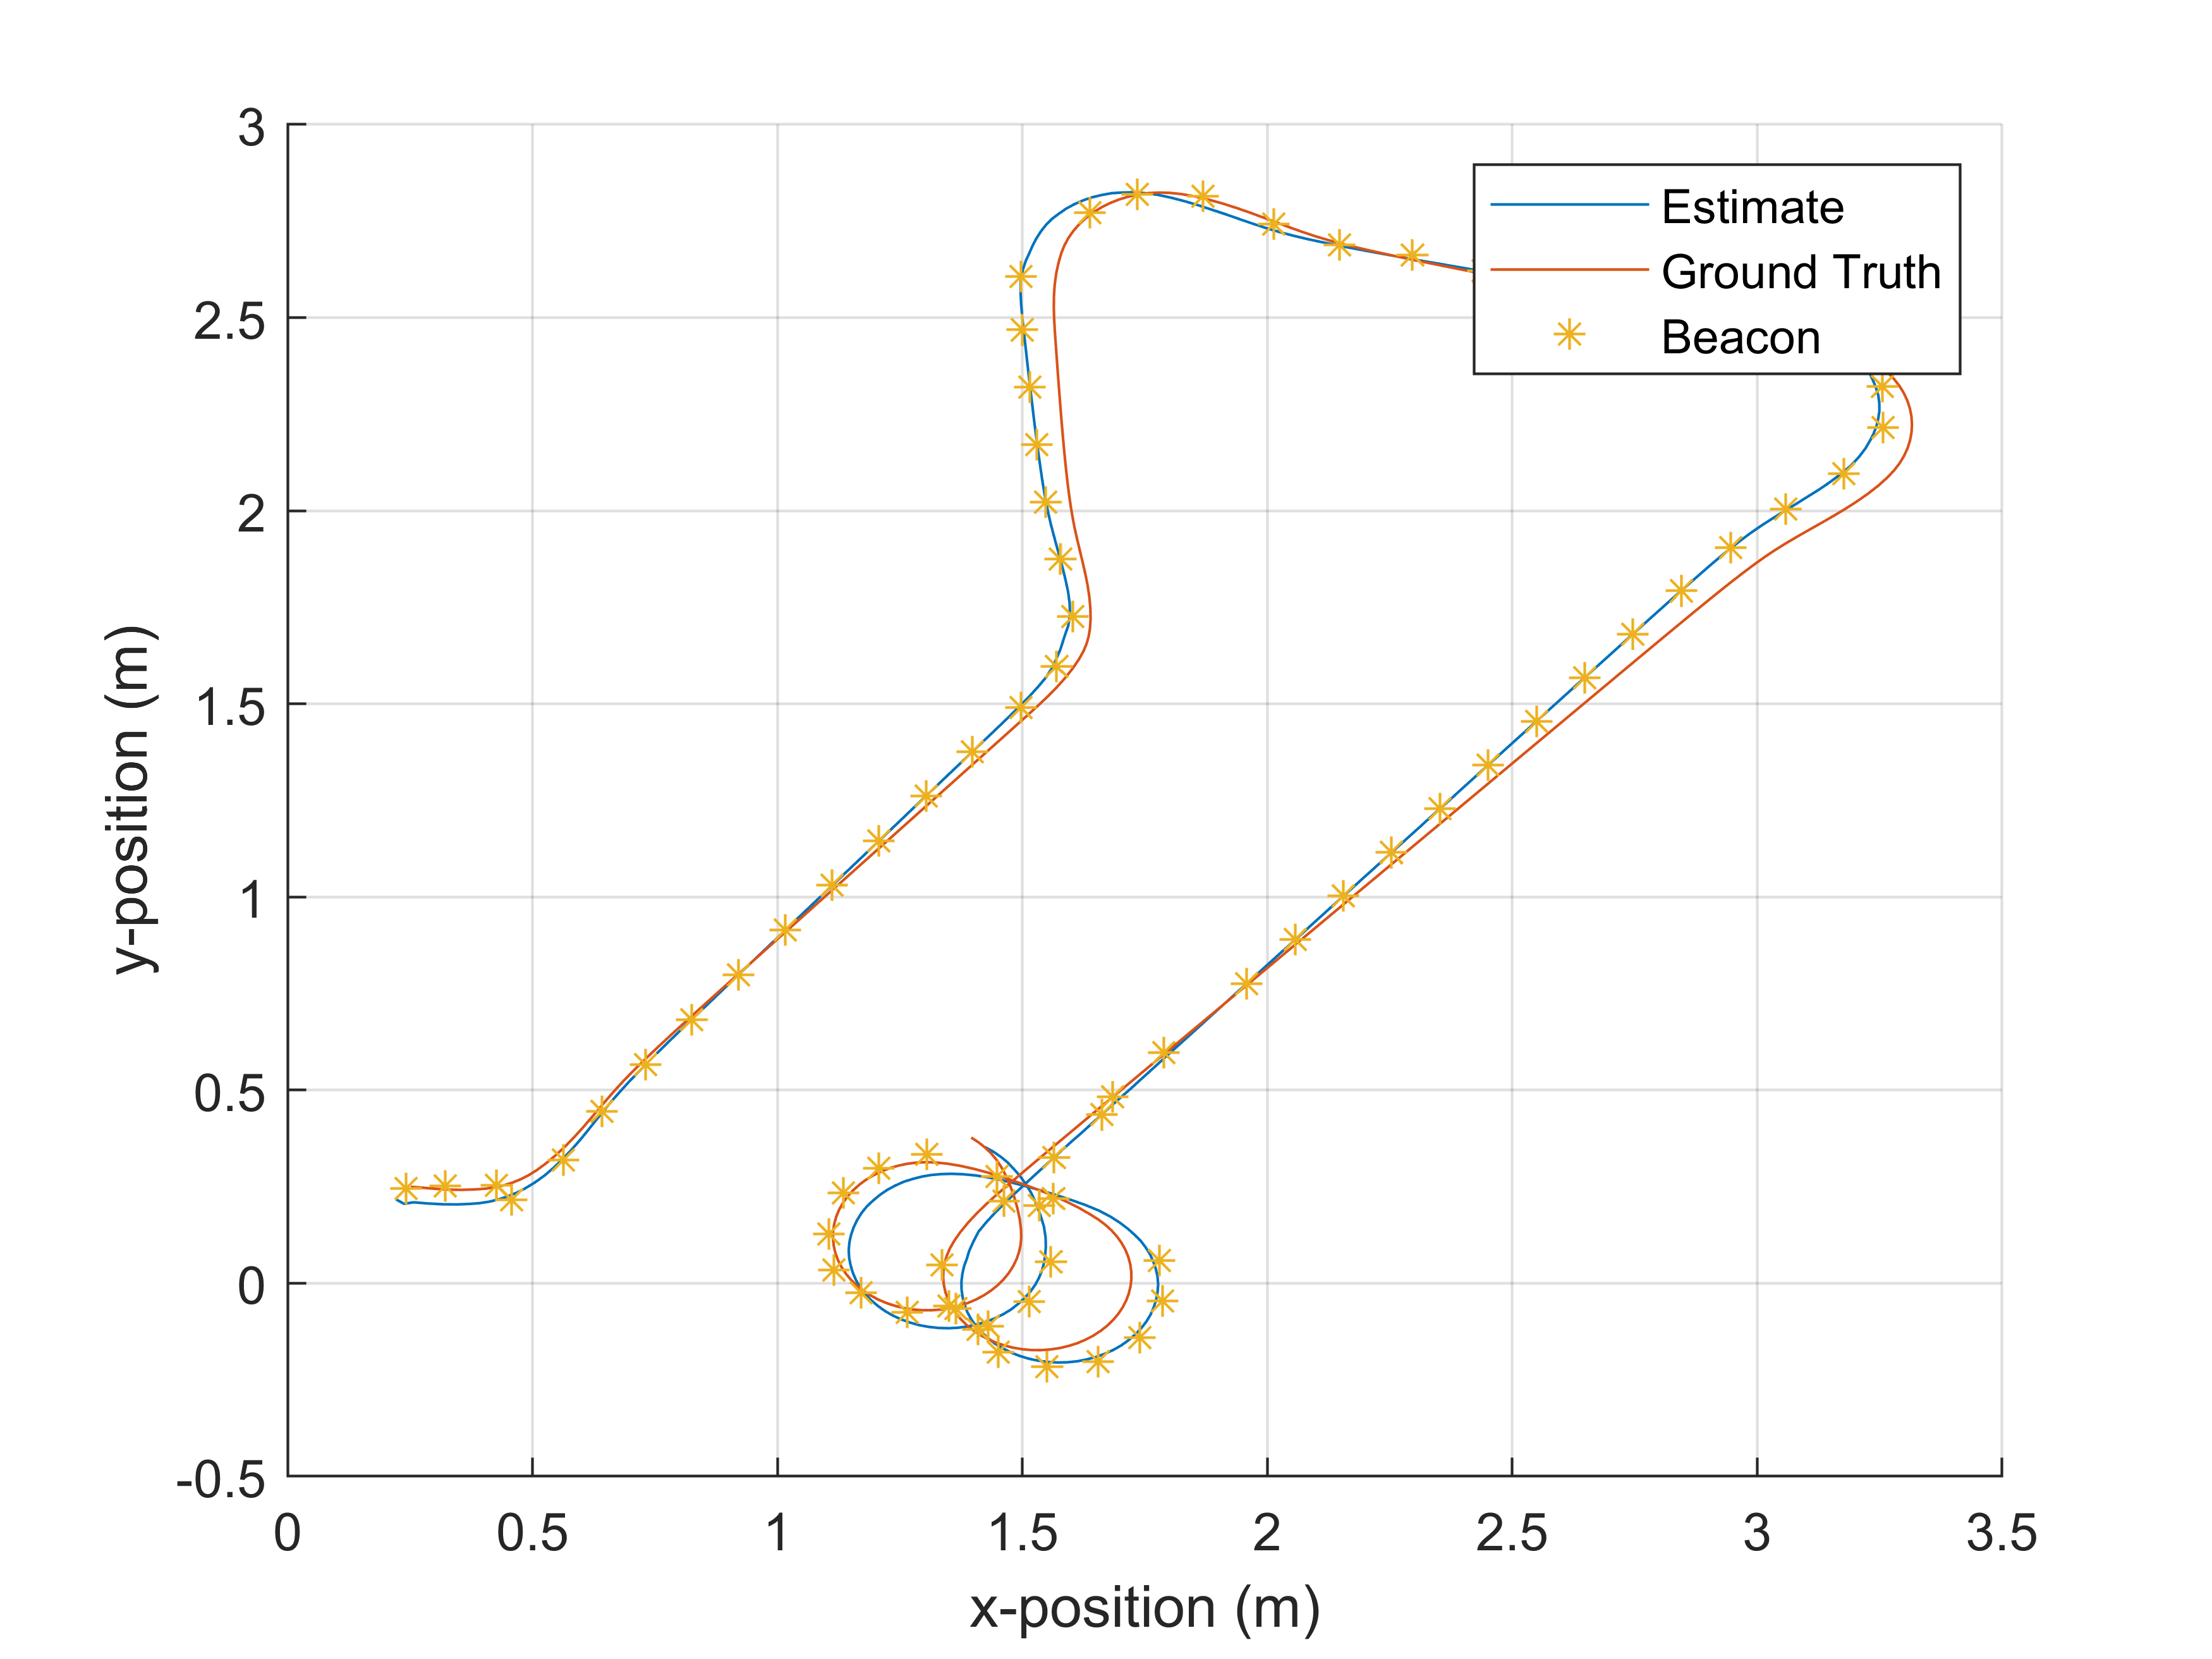
\includegraphics[width=\columnwidth]{./graphics/posSimu.png}
	   	\caption{Position estimates versus ground truth (Simulation).}
		\label{fig:pos}
	\end{figure}
	
	\begin{figure}
	    	\captionsetup{width=\columnwidth}
	   	\centering
	   	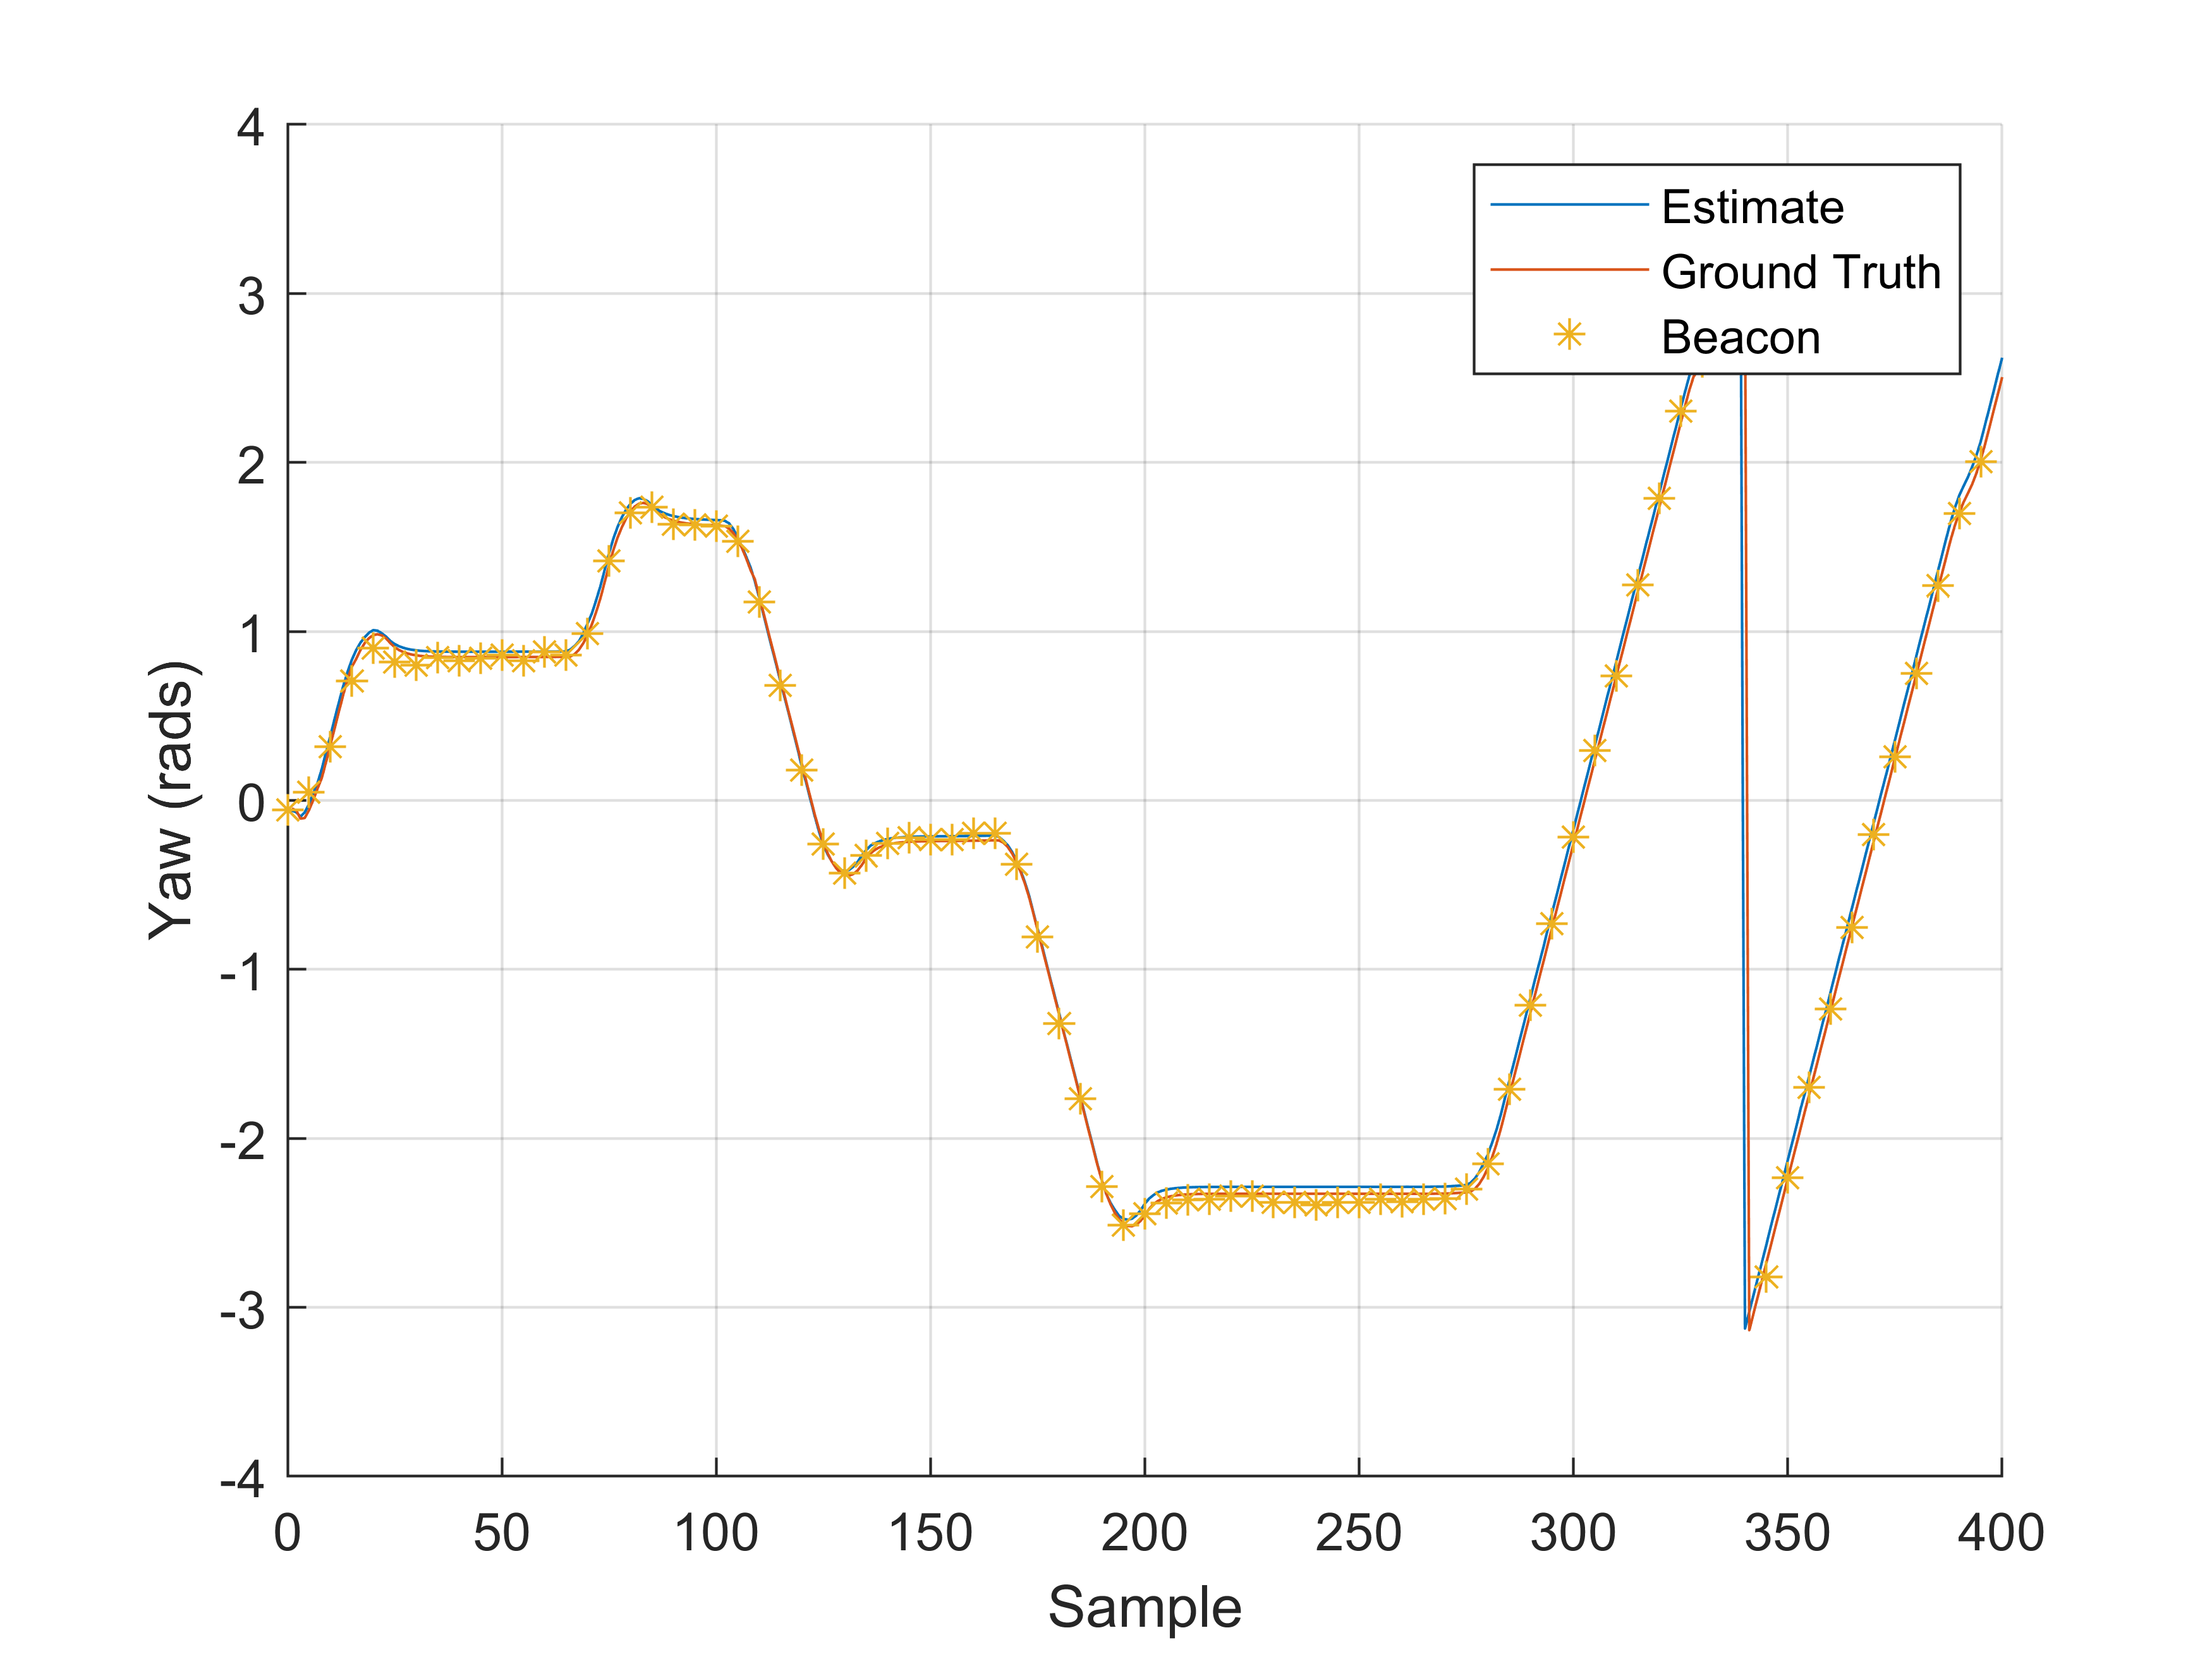
\includegraphics[width=\columnwidth]{./graphics/yawSimu.png}
	   	\caption{Yaw estimates versus ground truth (Simulation.}
		\label{fig:yaw}
	\end{figure}
	
	\begin{figure}
	    	\captionsetup{width=\columnwidth}
	   	\centering
	   	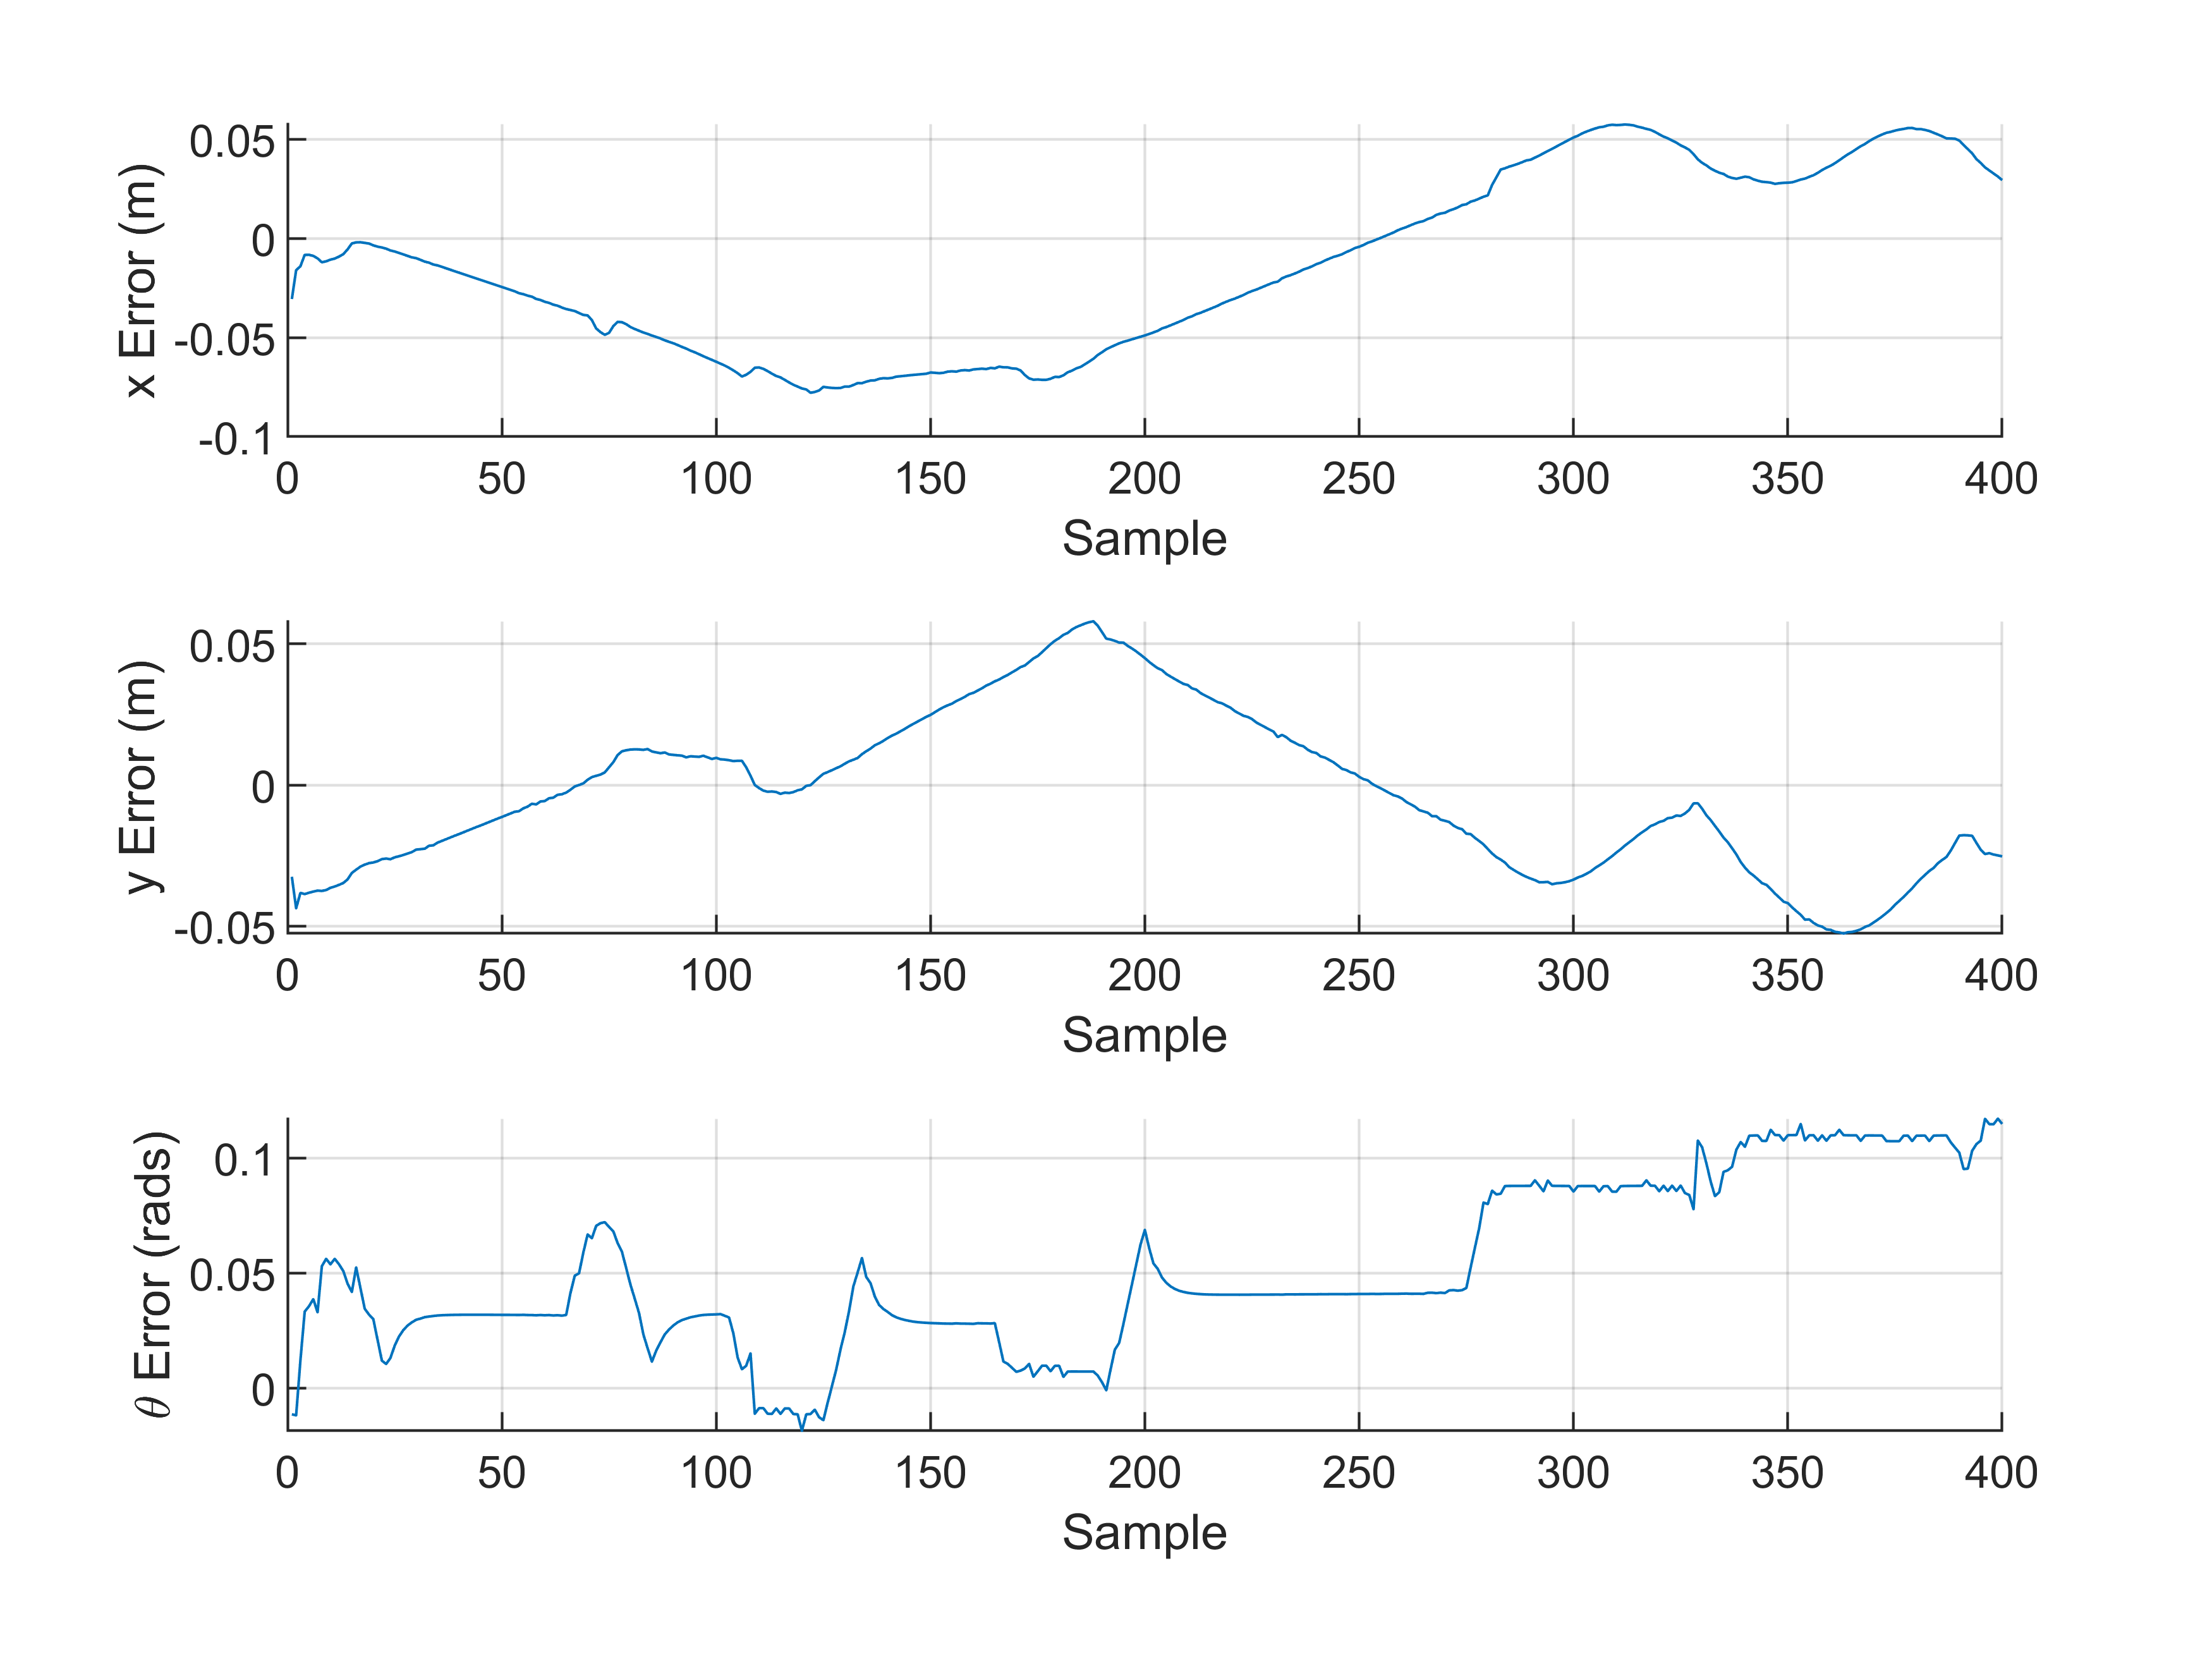
\includegraphics[width=\columnwidth]{./graphics/Error.png}
	   	\caption{Error plot of figure \ref{fig:pos} and \ref{fig:way}.}
		\label{fig:err2}
	\end{figure}
\FloatBarrier
\section{Conclusion}
\label{sec:con}
	In simulation, the method used above showed very promising results, with its biggest downfalls showing the possibility of being rectified. The systemic error in the state estimates was not due to the filtering process itself, and such should be fixable with a more accurate model of how the LiDAR works both in simulation and physically. The other issue was that of the update rate of the filter, due to the experiment being run entirely within MATLAB with local parallel processes, as well as the simulation running in a virtual machine running on the same machine, the fastest update rate achievable was 5Hz for the primary measurements, and 1Hz for the secondary. This was not a limitation of the dependent topics, as they updated at a rate of at least 25Hz based off initial tests. If the code was written in something like Python, and the physical TurtleBot used instead of the simulation, the processing could be more easily paralleled and distributed to offload the computation.\par
The methods as they stand are suitable as are as part of a more complex path planning and motion control algorithms as long as the systemic errors mentioned are taken into account for tolerances.

	\bibliographystyle{ieeetran}
	\bibliography{./sections/references.bib}
	
\begin{IEEEbiography}[{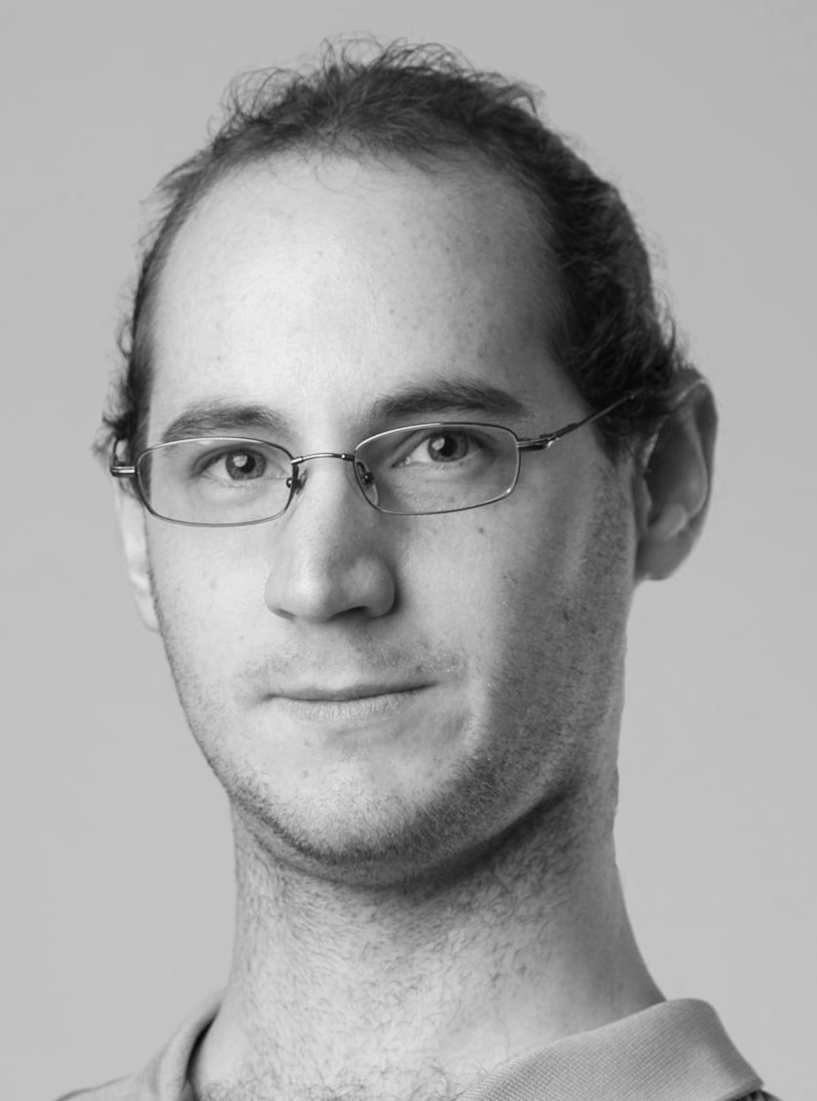
\includegraphics[width=1in,height=1.25in,clip,keepaspectratio]{a1.png}}]{Michael J. Duke} is was born in Adelaide, Australia in 1991. He is currently studying to receive the BEng(Hons) degree in mechatronic engineering for University of South Australia, Adelaide, Australia.\par
From 2009 to 2019, he held a full-time position as a Precision Agriculture Technician for Rocky River Ag Services in Crystal Brook, Australia. Since 2019, he has been working as a Mechatronic Design Engineer Undergraduate for Applidyne Australia Pty Ltd. in Adelaide, Australia. His current research interests include control systems, model based design and digital twins, and electric vehicle drive train and battery technology.
\end{IEEEbiography}

\EOD

\end{document}
